\documentclass[twoside]{book}

% Packages required by doxygen
\usepackage{fixltx2e}
\usepackage{calc}
\usepackage{doxygen}
\usepackage[export]{adjustbox} % also loads graphicx
\usepackage{graphicx}
\usepackage[utf8]{inputenc}
\usepackage{makeidx}
\usepackage{multicol}
\usepackage{multirow}
\PassOptionsToPackage{warn}{textcomp}
\usepackage{textcomp}
\usepackage[nointegrals]{wasysym}
\usepackage[table]{xcolor}

% Font selection
\usepackage[T1]{fontenc}
\usepackage[scaled=.90]{helvet}
\usepackage{courier}
\usepackage{amssymb}
\usepackage{sectsty}
\renewcommand{\familydefault}{\sfdefault}
\allsectionsfont{%
  \fontseries{bc}\selectfont%
  \color{darkgray}%
}
\renewcommand{\DoxyLabelFont}{%
  \fontseries{bc}\selectfont%
  \color{darkgray}%
}
\newcommand{\+}{\discretionary{\mbox{\scriptsize$\hookleftarrow$}}{}{}}

% Page & text layout
\usepackage{geometry}
\geometry{%
  a4paper,%
  top=2.5cm,%
  bottom=2.5cm,%
  left=2.5cm,%
  right=2.5cm%
}
\tolerance=750
\hfuzz=15pt
\hbadness=750
\setlength{\emergencystretch}{15pt}
\setlength{\parindent}{0cm}
\setlength{\parskip}{3ex plus 2ex minus 2ex}
\makeatletter
\renewcommand{\paragraph}{%
  \@startsection{paragraph}{4}{0ex}{-1.0ex}{1.0ex}{%
    \normalfont\normalsize\bfseries\SS@parafont%
  }%
}
\renewcommand{\subparagraph}{%
  \@startsection{subparagraph}{5}{0ex}{-1.0ex}{1.0ex}{%
    \normalfont\normalsize\bfseries\SS@subparafont%
  }%
}
\makeatother

% Headers & footers
\usepackage{fancyhdr}
\pagestyle{fancyplain}
\fancyhead[LE]{\fancyplain{}{\bfseries\thepage}}
\fancyhead[CE]{\fancyplain{}{}}
\fancyhead[RE]{\fancyplain{}{\bfseries\leftmark}}
\fancyhead[LO]{\fancyplain{}{\bfseries\rightmark}}
\fancyhead[CO]{\fancyplain{}{}}
\fancyhead[RO]{\fancyplain{}{\bfseries\thepage}}
\fancyfoot[LE]{\fancyplain{}{}}
\fancyfoot[CE]{\fancyplain{}{}}
\fancyfoot[RE]{\fancyplain{}{\bfseries\scriptsize Generated by Doxygen }}
\fancyfoot[LO]{\fancyplain{}{\bfseries\scriptsize Generated by Doxygen }}
\fancyfoot[CO]{\fancyplain{}{}}
\fancyfoot[RO]{\fancyplain{}{}}
\renewcommand{\footrulewidth}{0.4pt}
\renewcommand{\chaptermark}[1]{%
  \markboth{#1}{}%
}
\renewcommand{\sectionmark}[1]{%
  \markright{\thesection\ #1}%
}

% Indices & bibliography
\usepackage{natbib}
\usepackage[titles]{tocloft}
\setcounter{tocdepth}{3}
\setcounter{secnumdepth}{5}
\makeindex

% Hyperlinks (required, but should be loaded last)
\usepackage{ifpdf}
\ifpdf
  \usepackage[pdftex,pagebackref=true]{hyperref}
\else
  \usepackage[ps2pdf,pagebackref=true]{hyperref}
\fi
\hypersetup{%
  colorlinks=true,%
  linkcolor=blue,%
  citecolor=blue,%
  unicode%
}

% Custom commands
\newcommand{\clearemptydoublepage}{%
  \newpage{\pagestyle{empty}\cleardoublepage}%
}

\usepackage{caption}
\captionsetup{labelsep=space,justification=centering,font={bf},singlelinecheck=off,skip=4pt,position=top}

%===== C O N T E N T S =====

\begin{document}

% Titlepage & ToC
\hypersetup{pageanchor=false,
             bookmarksnumbered=true,
             pdfencoding=unicode
            }
\pagenumbering{alph}
\begin{titlepage}
\vspace*{7cm}
\begin{center}%
{\Large My Project \\[1ex]\large \#\+Harsheys }\\
\vspace*{1cm}
{\large Generated by Doxygen 1.8.14}\\
\end{center}
\end{titlepage}
\clearemptydoublepage
\pagenumbering{roman}
\tableofcontents
\clearemptydoublepage
\pagenumbering{arabic}
\hypersetup{pageanchor=true}

%--- Begin generated contents ---
\chapter{Hierarchical Index}
\section{Class Hierarchy}
This inheritance list is sorted roughly, but not completely, alphabetically\+:\begin{DoxyCompactList}
\item Q\+Main\+Window\begin{DoxyCompactList}
\item \contentsline{section}{Main\+Window}{\pageref{class_main_window}}{}
\end{DoxyCompactList}
\end{DoxyCompactList}

\chapter{Class Index}
\section{Class List}
Here are the classes, structs, unions and interfaces with brief descriptions\+:\begin{DoxyCompactList}
\item\contentsline{section}{\mbox{\hyperlink{class_main_window}{Main\+Window}} }{\pageref{class_main_window}}{}
\item\contentsline{section}{\mbox{\hyperlink{class_plotter}{Plotter}} }{\pageref{class_plotter}}{}
\end{DoxyCompactList}

\chapter{Class Documentation}
\hypertarget{class_main_window}{}\section{Main\+Window Class Reference}
\label{class_main_window}\index{Main\+Window@{Main\+Window}}
Inheritance diagram for Main\+Window\+:\begin{figure}[H]
\begin{center}
\leavevmode
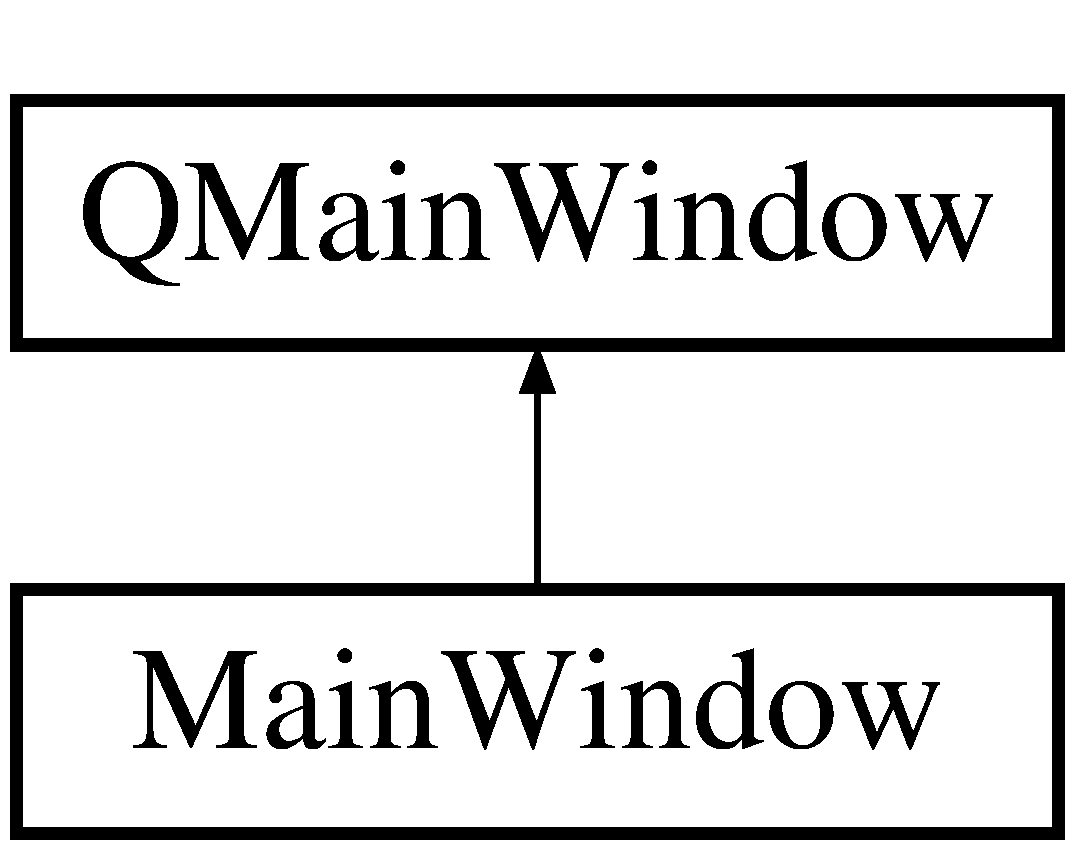
\includegraphics[height=2.000000cm]{class_main_window}
\end{center}
\end{figure}
\subsection*{Public Slots}
\begin{DoxyCompactItemize}
\item 
\mbox{\Hypertarget{class_main_window_afdfeb13ec363b0eb8ecacaf0aa13b605}\label{class_main_window_afdfeb13ec363b0eb8ecacaf0aa13b605}} 
void {\bfseries put\+Data} ()
\item 
\mbox{\Hypertarget{class_main_window_aea419351969ceb1745bce8c32cc40898}\label{class_main_window_aea419351969ceb1745bce8c32cc40898}} 
void {\bfseries Connecttcp} ()
\item 
\mbox{\Hypertarget{class_main_window_ad194178551f1276153573dadbd16cfe4}\label{class_main_window_ad194178551f1276153573dadbd16cfe4}} 
void {\bfseries Disconnecttcp} ()
\item 
\mbox{\Hypertarget{class_main_window_a380872c4aa4095322c798c8ea0ed357e}\label{class_main_window_a380872c4aa4095322c798c8ea0ed357e}} 
void {\bfseries set\+Timing} ()
\item 
\mbox{\Hypertarget{class_main_window_a6c6f436be38f1b757ca1378596e4f65d}\label{class_main_window_a6c6f436be38f1b757ca1378596e4f65d}} 
void {\bfseries Temp\+ON} ()
\item 
\mbox{\Hypertarget{class_main_window_a4c7f4a0aea66c32ce97ad252109b4247}\label{class_main_window_a4c7f4a0aea66c32ce97ad252109b4247}} 
void {\bfseries Temp\+O\+FF} ()
\item 
\mbox{\Hypertarget{class_main_window_a748efcbe7c110e645ecebf7aae442879}\label{class_main_window_a748efcbe7c110e645ecebf7aae442879}} 
void {\bfseries set\+Maximo} ()
\item 
\mbox{\Hypertarget{class_main_window_a65f18a0fb5579ff98e4f95aab314cf88}\label{class_main_window_a65f18a0fb5579ff98e4f95aab314cf88}} 
void {\bfseries set\+Minimo} ()
\end{DoxyCompactItemize}
\subsection*{Public Member Functions}
\begin{DoxyCompactItemize}
\item 
\mbox{\Hypertarget{class_main_window_a8b244be8b7b7db1b08de2a2acb9409db}\label{class_main_window_a8b244be8b7b7db1b08de2a2acb9409db}} 
{\bfseries Main\+Window} (Q\+Widget $\ast$parent=0)
\item 
\mbox{\Hypertarget{class_main_window_aaa425b1554af3c1f58cc70b4815082ae}\label{class_main_window_aaa425b1554af3c1f58cc70b4815082ae}} 
void {\bfseries timer\+Event} (Q\+Timer\+Event $\ast$event)
\end{DoxyCompactItemize}


The documentation for this class was generated from the following files\+:\begin{DoxyCompactItemize}
\item 
mainwindow.\+h\item 
mainwindow.\+cpp\end{DoxyCompactItemize}

\hypertarget{class_plotter}{}\section{Plotter Class Reference}
\label{class_plotter}\index{Plotter@{Plotter}}
Inheritance diagram for Plotter\+:\begin{figure}[H]
\begin{center}
\leavevmode
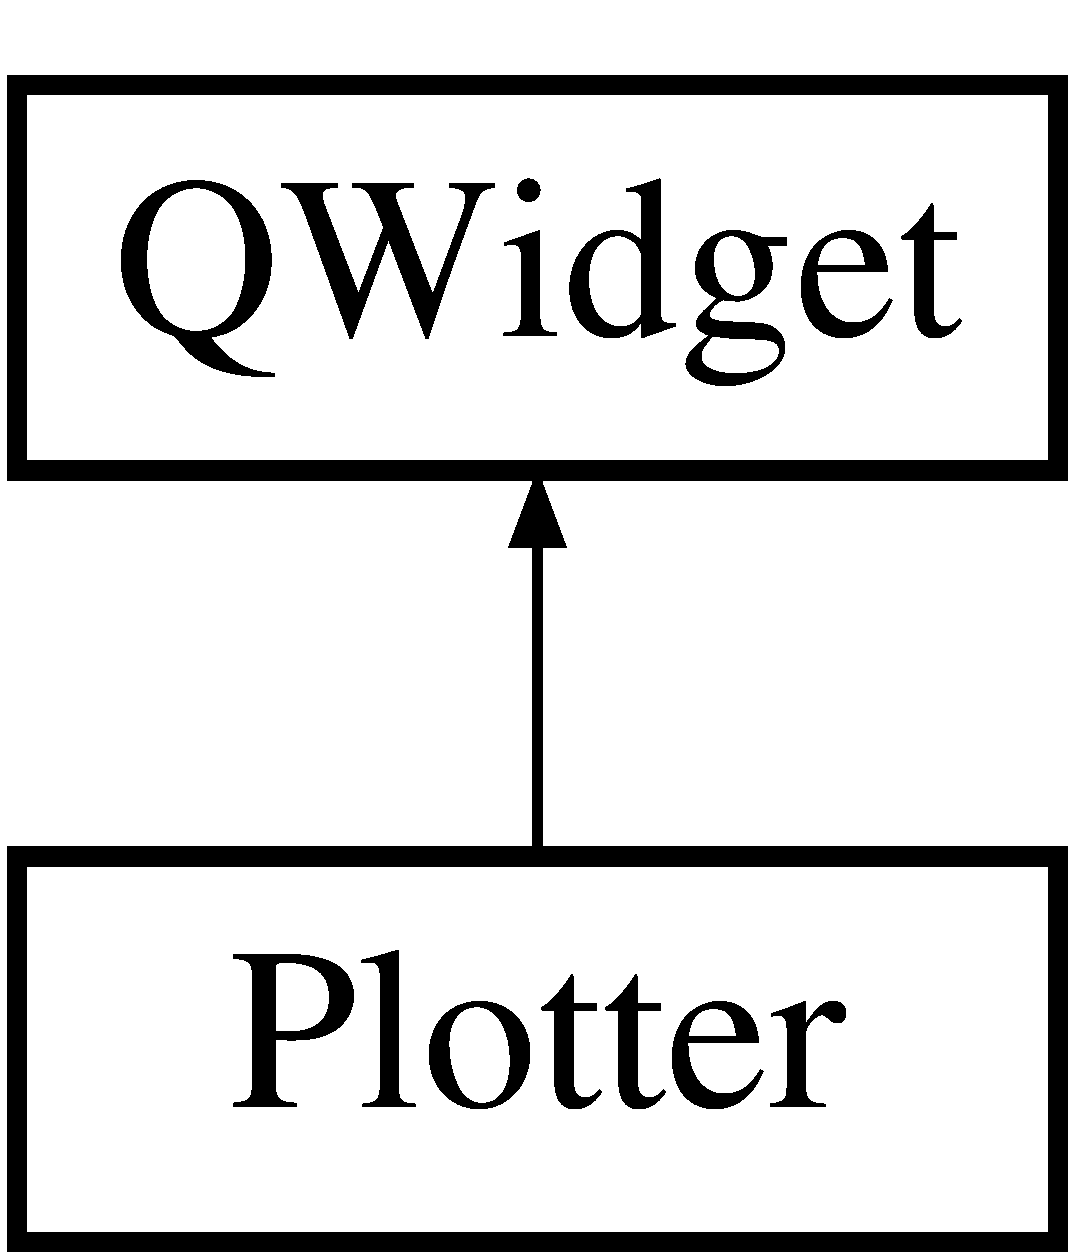
\includegraphics[height=2.000000cm]{class_plotter}
\end{center}
\end{figure}
\subsection*{Public Slots}
\begin{DoxyCompactItemize}
\item 
\mbox{\Hypertarget{class_plotter_a836f9d98817e7e4226fe41fbe4ea2a87}\label{class_plotter_a836f9d98817e7e4226fe41fbe4ea2a87}} 
void \mbox{\hyperlink{class_plotter_a836f9d98817e7e4226fe41fbe4ea2a87}{new\+Pontos}} (Q\+List$<$ int $>$ novosP)
\begin{DoxyCompactList}\small\item\em new\+Pontos é o método responsável por atualizar a lista de pontos definida na variável pontos. \end{DoxyCompactList}\item 
\mbox{\Hypertarget{class_plotter_a3dcb7c8bf30d03f0c0c8e2be14b83f58}\label{class_plotter_a3dcb7c8bf30d03f0c0c8e2be14b83f58}} 
int \mbox{\hyperlink{class_plotter_a3dcb7c8bf30d03f0c0c8e2be14b83f58}{p\+Max}} ()
\begin{DoxyCompactList}\small\item\em p\+Max retorna o índice do maior número na lista de pontos. \end{DoxyCompactList}\item 
\mbox{\Hypertarget{class_plotter_a6196ac5880e4cdb9c2b2145678927f73}\label{class_plotter_a6196ac5880e4cdb9c2b2145678927f73}} 
int \mbox{\hyperlink{class_plotter_a6196ac5880e4cdb9c2b2145678927f73}{p\+Min}} ()
\begin{DoxyCompactList}\small\item\em p\+Min retorna o índice do menor número na lista de pontos. \end{DoxyCompactList}\end{DoxyCompactItemize}
\subsection*{Public Member Functions}
\begin{DoxyCompactItemize}
\item 
\mbox{\Hypertarget{class_plotter_a1807627530de30ae58dff3c42a823497}\label{class_plotter_a1807627530de30ae58dff3c42a823497}} 
{\bfseries Plotter} (Q\+Widget $\ast$parent=nullptr)
\item 
\mbox{\Hypertarget{class_plotter_a06477bf987646f000a8982db1352a11d}\label{class_plotter_a06477bf987646f000a8982db1352a11d}} 
void {\bfseries paint\+Event} (Q\+Paint\+Event $\ast$event)
\end{DoxyCompactItemize}


The documentation for this class was generated from the following files\+:\begin{DoxyCompactItemize}
\item 
plotter.\+h\item 
plotter.\+cpp\end{DoxyCompactItemize}

%--- End generated contents ---

% Index
\backmatter
\newpage
\phantomsection
\clearemptydoublepage
\addcontentsline{toc}{chapter}{Index}
\printindex

\end{document}
